\documentclass[letterpaper]{llncs}

\title{RoboCup Small-Size\\Execution Flow and Timing}
\author{Roman Shtylman\\\email{shtylman@gmail.com}}
\institute{Georgia Institute of Technology}

\usepackage{graphicx}

\begin{document}

\maketitle

\begin{abstract}
When controlling robots in a real-time environment, understanding the execution order and timing for the system is critical. In order to perform reliable control in a closed loop, the timings from iteration to iteration should be as consistent and deterministic as possible. Minimizing the latency is also critical, and, in a game-play environment, the robots should respond as fast as possible. This creates a trade-off between having low latency, consistent timing, and reduced implementation complexity. The focus of this project is to design such a system and describe how it provides consistent timing and low latency.
\end{abstract}

\section{Problem Overview}
RoboCup is an international robotics competition with the goal of developing a team of robots that, by 2050, can defeat the world championship human soccer team. The competition is divided into different leagues, differentiated by robot size and capabilities. Small-Size League works with teams of robots that have, at most, a 180mm diameter footprint and a height of 150 mm. A team consists of up to five of these robots. A central computer controls the actions of the robots; this includes setting goals, planning a path, and communicating over radios to drive them. The computer is also connected to cameras over the field which are used for locating the robots and ball. Once gameplay has begun, the entire system must act autonomously with no human interaction as the robots play each of their 10 minute halves.

There are no restrictions on the number or capabilities of the overhead cameras, but most teams use two, one over each half of the field. Teams can use any capture technology they wish to acquire the frames. Most employ either firewire or gigE (network) connectivity. After vision processing of the frames, teams have various forms of control and gameplay that creates commands for a radio to transmit packets to/from the robots. Often, this is one computer that is able to handle the entire computational load, but again there are no restrictions and some teams use multiple computers.

The robots themselves are often simple from a software perspective. They simply execute basic commands (i.e. spinning motors at a certain speed). Robots can also have sensors that relay information back to the system (i.e. ball presence, battery health). Again, there are no restrictions or limitations and teams are free to add any capabilities they see fit so long as the robot stay within dimension and do not exceed the maximum kick speed.

\subsection{RoboJackets}
The RoboJackets have competed in RoboCup events for two years, starting with the international event in 2007. We have fielded two different sets of robots each year as well as different software and cameras. This provides the experience and base for redesigning the 2009 system. The 2007 and 2008 systems will not be discussed here for brevity, instead, only the 2009 system and its rationale will be covered. This document will only cover the software aspects and ignore the mechanical and electrical.

\section{System Components}
Our general approach matches that of other teams. In 2007, we had two overhead firewire cameras running at 60fps and a radio base station using serial to communicate with the computer. In 2008, we again had two overhead cameras (gigE) running at 90 fps and a radio capable of talking to the robots at the same speed. All teams will share this common infrastructure of cameras, processing, and radio. 

We have separated the components, based on their hardware requirements, into three categories: vision, radio, and processing.

\subsection{Vision}
The vision system is the first step before any control or gameplay can occur. Vision is responsible for capturing frames from the camera(s) and processing them for robot pose information. After a frame has been processed, a list of potential ball locations and robots is created. This information is then passed to the rest of the system for further usage. The rest of the system relies on knowing where the robots and ball are before continuing.

This simple pre-requisite sets up the basis for our design of the rest of the system. Because vision is something that comes it at a fixed interval and tells us the ``truth'' about the world, we base all of our other processes on it. The framerate (rate at which the camera is able to capture frames) becomes the baseline timing interval from which other processes are measured against. Framerate and frame interval (time between camera frames) are both important metrics used to make design decisions.

\subsection{Radio}
The radio hardware design is outside the scope of this paper and much of the information described about the radios is already present in current prototypes and is reproduced here for describing how it will integrate with the rest of the system.

%%%%%% verify the actual radio cycle time
The radio hardware connects to a host computer through USB. This creates a variable latency from 0 to 1ms to send packets to and from from the radio hardware. This latency depends on when USB is polled by the system and is at most 1ms. Another variable latency of at most 9ms is also present for sending data to/from the robots on the field. Both send and receive occur during this period. And new data from the robots is only available at the end of this period.

\subsection{Processing}
Processing describes anything that is not directly tied to communicating with hardware. This includes decision making for gameplay, world model creation, motion control, and so forth. There are two types of processing: synchronous and asynchronous. The reasoning for this division will be described in more detail in the upcoming sections as well as the flow and timing description.

\subsubsection{Synchronous Processing}
Synchronous processing is required to occur as a result of vision processing finishing. Once vision information is available, items like the world model and motion control can be updated with the latest real pose information. Because these processes are guaranteed to occur between frames and once every cycle, they should not block or take an excessively long time. Motion control is performed as a synchronous process. This allows motion control to run with the latest realworld information as soon as it becomes available and have robot commands ready for the next transmission cycle.

\subsubsection{Asynchronous Processing}
Asynchronous processing is not required to occur as a result of vision processing finishing nor must it finish before the next frame arrives. It is used for higher level decisions that may take longer than a frame interval to process. Certain system states will not change with every frame change and therefore do not need to be processed every frame. Asynchronous processing exists for such tasks and is performed independently of other processes.

\section{System Design and Integration}
This section focuses on how the various components interact and integrate with one another in the overall system framework. It also covers the execution order and further details about the system from a runtime perspective.

\subsection{Components Revisited}
The three major components were separated above to display their unique roles with respect to hardware. One system integration possibility is to have all of the components residing in one application running on one computer capable of performing all the required tasks. While simple to implement, this makes the end result very inflexible. The hardware only dictates that vision run on the same computer as a camera is sending frames to; likewise, the radio process must be able to physically talk to the radio and must also run on the computer the radio hardware is connected to. This does not limit the two processes to one machine. Likewise, our system does not improse such a limitation, but instead allows each of the three major components to run independently of each other and communicate using a define interface.

Because interfaces limit functionality, we are careful in how many divisions we create and limit ourselves to just the ones that have clear distinctions and add flexibility without being too restrictive. By separating hardware based processes from pure software ones, we can easily replace the hardware components with simulations without changing the interface to pure software components. This allows us to perform a wider range of tests using more controlled environments, i.e. a simulator, when testing the execution flow and timing.

\section{Execution}

\subsection{Execution Flow}
An execution cycle is defined as the process of grabbing a camera frame, performing vision processing, performing control processing, and then sending out the radio data. The information will happen in that exact order, meaning that processing must wait for vision to finish, and radio must wait for processing to finish before being able to send new data.

Because having a consistent processing and radio transmit interval is important from a controls perspective, we use the arrival of a frame as a synchronization point. \textbf{Figure \ref{execflow}} shows a sample one camera execution environment.

\begin{figure}[h]
	\centering
	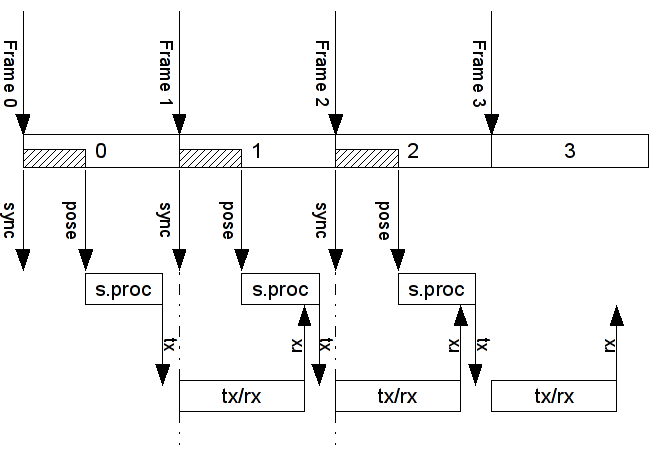
\includegraphics[width=.75\textwidth]{images/execflow.png}
	\caption{one camera execution flow}
	\label{execflow}
\end{figure}

The top row shows the frames arriving from the camera. Each numbered box represents a new frame. The space between frames (width of the box) is the frame interval. Once a frame arrives, a \textit{sync} message is sent to notify the system of its arrival; because the frames arrive at a fixed interval, this \textit{sync} message timing is fixed and can be relied on as a base for other timing critical tasks.

The hashed regions in each frame shows the vision processing. After processing is complete, pose information is available and synchronous processes can run. The result of synchronous processes is commands that can be sent over the radio to the robots for closed loop control. This information must be available before the next frame arrives. Each time a \textit{sync} message is received by the radio process, the last available command is sent and new data is received from the robots. This new data is available after the tx/rx cycle is complete. As clearly shown, this means that synchronous processing during one cycle uses the current available vision information and one frame delay on radio information (frame 2's \textit{s.proc} is actually using radio information received during frame 1's \textit{tx/rx} cycle).

Synchronous processes, specifically control code to generate robot commands, must complete on time with room to spare for any communication delays. The \textit{tx/rx} bar includes the usb delay as well as the actual radio transmit/receive cycle. 

Radio data is transmitted at the \textit{sync} message boundary instead of the completion of \textit{s.proc} to ensure that radio data is sent at a fixed interval; vision processing and synchronous processing times may vary and we do not want radio transmission to be affected by this variation.

\subsection{Two Camera Execution}
When running with two (or more cameras) the basic execution flow is preserved with some added delays to account for frames that arrive at a fixed offset from different cameras. To keep the system simple, we want to have all of the vision information before proceeding with any synchronous processing (full field coverage). This means that when processing multiple frames, we need to wait until the \textit{trigger} camera reports a frame arrival.

\subsubsection{Trigger Camera}
The \textit{trigger} camera is defined to be the last camera to report a frame. The worst case difference between frame times is $\frac{1}{2}$ a frame interval, and the best case is to have the cameras synchronized thus making the delay negligible. Regardless of the delay, the same execution flow is observed. Each camera has its own vision process that reports a \textit{sync} message when a frame arrives and a \textit{pose} message when vision processing is complete.

If, when the cameras are started, the second camera frame arrives after $\frac{1}{2}$ of the first camera's frame interval has passed, the second camera becomes the trigger camera. This ensures that the overall latency incurred from offset frame arrivals is at most $\frac{1}{2}$ frame interval. \textbf{Figure \ref{largeoffset}} shows that \textit{camera 1} becomes the trigger camera and thus reduces the latency. Frame 0 is dropped.

\begin{figure}[h]
	\centering
	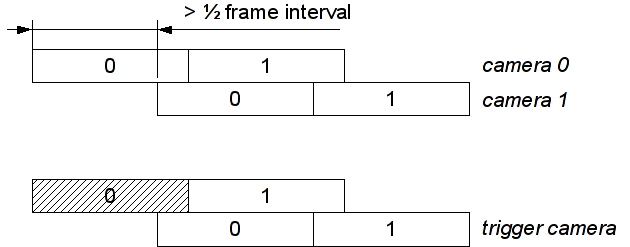
\includegraphics[width=.75\textwidth]{images/largeoffset.png}
	\caption{correcting large offset}
	\label{largeoffset}
\end{figure}

\pagebreak

After the \textit{trigger} camera is chosen, the execution is the same as single camera with respect to the \textit{trigger} camera. The only difference between one and two cameras is the added complexity in any processing to track robots between cameras and determine where objects really are between the two frames. This is all done after receiving the information from both cameras.

\begin{figure}[h]
	\centering
	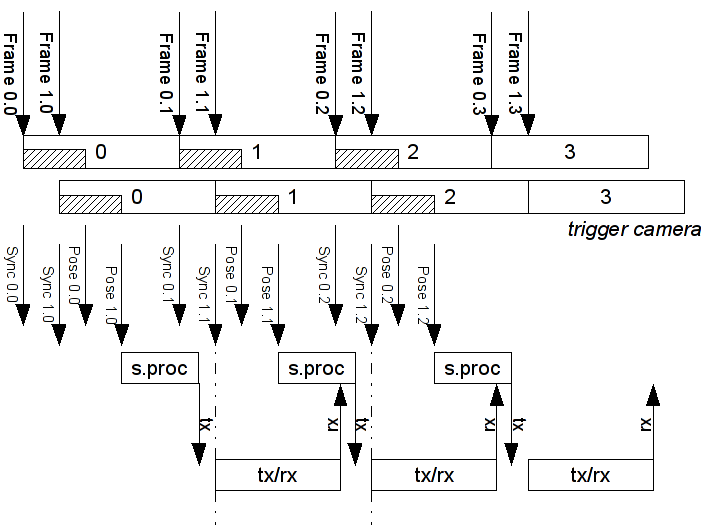
\includegraphics[width=.75\textwidth]{images/two_camera.png}
	\caption{two camera execution flow}
	\label{twocamera}
\end{figure}

\section{Validation}
In order to make sure that the system is running with the correct timing, we want to have a method for recording what happened and when. Each time there is a message between components we want to log the time. Because this logging needs to happen in a central location as be able to capture information for every cycle, we choose synchronous processing as the location for logging.

A log frame is all of the data from one cycle. It is written at the end of \textit{s.proc} once the robot command data is known. If we write the data out at that point we have all of the information that was used and created as a result of the latest \textit{trigger} frame. Notice, that the \textit{tx/rx} cycle finishes in the middle of \textit{s.proc} and its arrival time is logged when the \textit{rx} data arrives.

\subsection{Latencies}
Calculating the latencies can be done with all of the above logged information. Some example calculations are presented below for high concern items.

\begin{description}
\item [Radio cycle] \textit{(trigger sync time) - (rx time)}
\item [Vision Processing] \textit{(sync time 0.0) - (pose time 0.0)}
\item [Frame Offset] \textit{(sync 0.0) - (sync 1.0)}
\item [S. Processing] \textit{(trigger sync time) - (tx time)}
\end{description}

Other latencies and times can be calculated, but the above are ones that are most critical to system operation. Using the times, the system can be validated to show that \textit{s.proc} always finishes before the next \textit{trigger frame arrives} and that a radio cycle completes sometime during a frame interval.

\subsection{Testing}
For testing the system to make sure that it is performing as expected, we will use the logged information to display the latencies and other important timing factors. By calculating the latencies during runtime, or even during log playback and review, the system can flag frames and times that exceeded expected parameters. Event times are recorded when those events occur into the log frame, and thus, if we see that radio data was not available before the next \textit{sync} frame arrived, we know that our synchronous processing is taking too long. Similar reasoning can be applied to check other parts of the system. 

We can even aim to make the system robust to potential timing failures. If we can detect a timing failure, we can choose to drop or skip a frame of processing as well as alert the user of such a failure. During runtime, one skip might be enough to get the system back on track and still have the log data for later resolution of the problem.

\section{Conclusion}
The described system is a considerable improvement over the 2008 system. We have removed many unnessesary interfaces as well as defined specific order of execution, timing, and validation methods. In doing so, we have not placed too many constraints on the application and also allowed for expansion as well as taking advantage of hardware improvements, like synchronized cameras.

\end{document}